\documentclass[12pt]{article}
\usepackage[english]{babel}
\usepackage{natbib}
\usepackage{url}
\usepackage[utf8x]{inputenc}
\usepackage{amsmath}
\usepackage{graphicx}
\graphicspath{{img/}}
\usepackage{parskip}
\usepackage{fancyhdr}
\usepackage{listings}
\usepackage{vmargin}
\setmarginsrb{3 cm}{2.5 cm}{3 cm}{2.5 cm}{1 cm}{1 cm}{1 cm}{1 cm}

\title{Lab Report on \\Introduction to MATLAB }								% Title
\author{Rabi Raj Khadka }								% Author
\date{\today}											% Date


\makeatletter
\let\thetitle\@title
\let\theauthor\@author
\let\thedate\@date
\makeatother

\pagestyle{fancy}
\fancyhf{}
\rhead{\theauthor}
\lhead{\thetitle}
\cfoot{\thepage}

\begin{document}

%%%%%%%%%%%%%%%%%%%%%%%%%%%%%%%%%%%%%%%%%%%%%%%%%%%%%%%%%%%%%%%%%%%%%%%%%%%%%%%%%%%%%%%%%

\begin{titlepage}
	\centering
    \vspace*{0.2 cm}
    
\includegraphics[scale = 0.3]{kheclogo.jpg}\\[1.0 cm]	% University Logo
    \textsc{\LARGE Khwopa Engineering College}\\[2.0 cm]	% University Name
	\textsc{\Large Course Code :BEG 475 IP}\\[0.5 cm]				% Course Code
	\textsc{\large Image Processing and Pattern Recogntiion}\\[0.5 cm]				% Course Name
	\rule{\linewidth}{0.2 mm} \\[0.4 cm]
	{ \huge \bfseries \thetitle}\\
	\rule{\linewidth}{0.2 mm} \\[1.0 cm]
	% \texttt{Lab Report \#1}
	
	\rule{\linewidth}{0 mm} \\[1.0 cm]

	\begin{minipage}{0.4\textwidth}
		\begin{flushleft} \large
			\emph{Author:}\\
			\theauthor
			\end{flushleft}
			\end{minipage}~
			\begin{minipage}{0.4\textwidth}
			\begin{flushright} \large
			\emph{Roll  Number:} \\
			700324									% Your Student Number
		\end{flushright}
	\end{minipage}\\[2 cm]
	
	{\large \thedate}\\[2 cm]
 
	\vfill
	
\end{titlepage}

%%%%%%%%%%%%%%%%%%%%%%%%%%%%%%%%%%%%%%%%%%%%%%%%%%%%%%%%%%%%%%%%%%%%%%%%%%%%%%%%%%%%%%%%%

\tableofcontents
\pagebreak

%%%%%%%%%%%%%%%%%%%%%%%%%%%%%%%%%%%%%%%%%%%%%%%%%%%%%%%%%%%%%%%%%%%%%%%%%%%%%%%%%%%%%%%%%

\section{Theory:}
\subsection{MATLAB}
Matlab \\The Language of Technical Computing\\
Millions of engineers and scientists worldwide use MATLAB® to analyze and design the systems and products transforming our world. The matrix-based MATLAB language is the world's most natural way to express computational mathematics. Built-in graphics make it easy to visualize and gain insights from data. The desktop environment invites experimentation, exploration, and discovery. These MATLAB tools and capabilities are all rigorously tested and designed to work together.\\

MATLAB helps us to run our analyses on larger data sets, and scale up to clusters and clouds. MATLAB code can be integrated with other languages, enabling us to deploy algorithms and applications within web, enterprise, and production systems.\\


\subsection{Few Command and Statements}

1.clc\\
 clc clears all input and output from the Command Window display, giving you a "clean screen." After using clc, we cannot use the scroll bar to see the history of functions, but we still can use the up arrow key, ↑, to recall statements from the command history.\\\\
2.disp()\\
disp(X) displays the value of variable X without printing the variable name. Another way to display a variable is to type its name, which displays a leading "X =" before the value. If a variable contains an empty array, disp returns without displaying anything.\\\\
3.if \thinspace\thinspace elseif \thinspace\thinspace else \\
if expression, statements, end evaluates an expression, and executes a group of statements when the expression is true. An expression is true when its result is nonempty and contains only nonzero elements (logical or real numeric). Otherwise, the expression is false.\\
The elseif and else blocks are optional. The statements execute only if previous expressions in the if...end block are false. An if block can include multiple elseif blocks.\\\\
4.end\\
end terminates for, while, switch, try, if, and parfor statements. Without an end statement, for, while, switch, try, if, and parfor wait for further input. Each end is paired with the closest previous unpaired for, while, switch, try, if, or parfor and serves to delimit its scope.\\
end also marks the termination of a function, although in many cases it is optional. If your function contains one or more nested functions, then you must terminate every function in the file, whether nested or not, with end. This includes primary, nested, private, and local functions.\\\\
5.input()\\
x = input(prompt) displays the text in prompt and waits for the user to input a value and press the Return key. The user can enter expressions, like pi/4 or rand(3), and can use variables in the workspace.\\
If the user presses the Return key without entering anything, then input returns an empty matrix.\\
If the user enters an invalid expression at the prompt, then MATLAB® displays the relevant error message, and then redisplays the prompt.\\
str = input(prompt,'s') returns the entered text as a string, without evaluating the input as an expression.\\\\
6.fprintf()\\
fprintf(fileID,formatSpec,A1,...,An) applies the formatSpec to all elements of arrays A1,...An in column order, and writes the data to a text file. fprintf uses the encoding scheme specified in the call to fopen.\\\\
7.plot()\\
plot(X,Y) creates a 2-D line plot of the data in Y versus the corresponding values in X.\\\\
8.while\\
while expression, statements, end evaluates an expression, and repeats the execution of a group of statements in a loop while the expression is true. An expression is true when its result is nonempty and contains only nonzero elements (logical or real numeric). Otherwise, the expression is false.\\
\pagebreak

\section{Code Description}
Basic Mathematical operations using MATLAB\\
\lstinputlisting[language=Matlab]{labone.m}





\pagebreak

\section{Result and Discussion}
Input Numbers are taken from user and different mathematical operations like addition, subtraction, multiplication,division are performed and result are shown. For the Matrix Operation two 3 x 3  matrices A and B are made and Multiplication, Addition, Subtraction on those matrices is done and Submatrix of Matrix A is also shown to the user.\\
On User choice to plot the graph, the system generates the figure for sine curve with range 0 to 2*Pi\\\\
\emph{Output:}\\

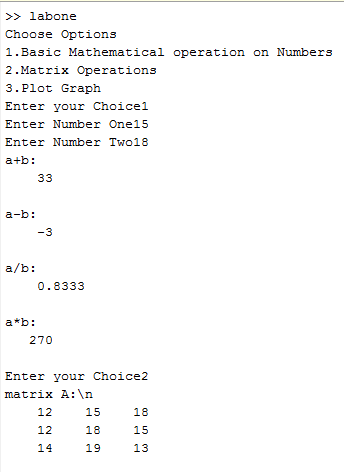
\includegraphics[scale =1.0]{output_labone_1.png}
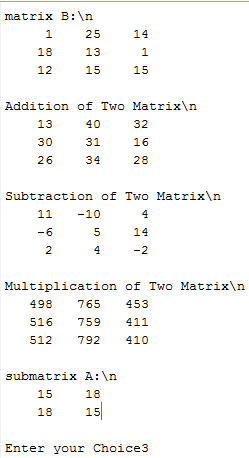
\includegraphics[scale =1.0]{output_labone_2.png}
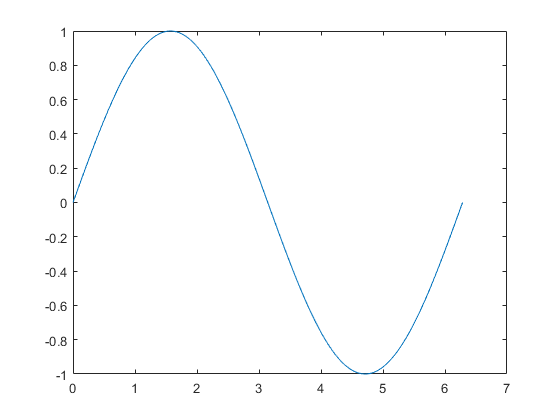
\includegraphics[scale =1.0]{output_labone_3.png}



\pagebreak

\section{Conclusion}
Hence, \\
We are familiarized with the MATLAB to perform basic programming and mathematical operation.
\newpage

\end{document}